% !TEXroot=main.tex
\section{Turtlebot}
{
	\subsection{Überblick}
	{
		Der Turtlebot ist ein beliebtes Robotermodell der Firma Robotis und kommt in verschiedenen Varianten. Das gute Preis-Leistungs-Verhältnis, sowie die Einsteigerfreundlichkeit, kombiniert mit vielen Integration in andere Programme machen in zu einer guten Wahl für viele Projekte
		Der Turtlebot 3 besteht aus vier Basisplatten, auf welchen die gesamte Technik des Roboters untergebracht ist. Auf der untersten Basisplatte findet man zwei Servomotoren der X-Series von Dynamixel vor, welche dem Turtlebot seine Mobilität verleihen, auf den anderen Plattformen ist ein Raspberry PI 3, welcher unter Umständen auch durch einen Raspberry Pi 4 ersetzt werden kann, sowie ein Einplatinencomputer vorzufinden. Bei Letzterem handelt es sich standardmäßig um einen Intel Joule 570x. Auf der obersten Basisplatte findet man Platz für einen Sensor vor, dort kann eine Kamera, allerdings auch ein Lasersensor oder ähnliches angebracht werden. Auf unserem Turtlebot ist ein LiDAR-Sensor montiert. Dieser Sensor sendet Laserimpulse aus und kann durch das zurückgestrahlte Licht den Raum exakt vermessen. Der Roboter tastet die Umgebung mit den Laserimpulsen ab, was dazu führt, dass er Messpunkte erhält. 
		
		\begin{figure}[H]
			\centering
			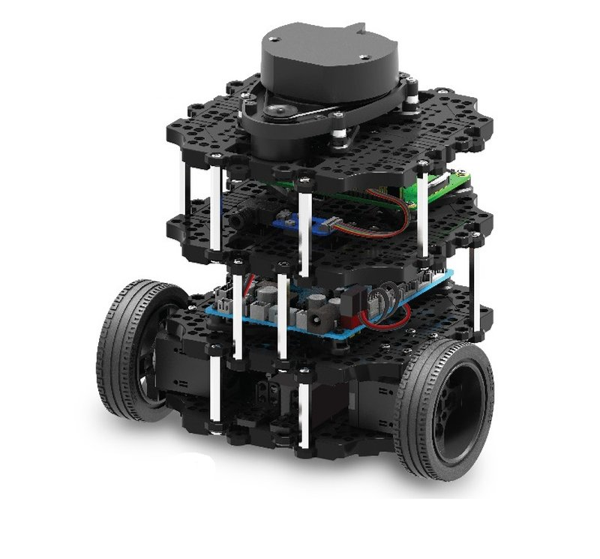
\includegraphics[height=5cm]{Bilder/turtlebot_3_burger.png}
			\caption{Der Turtlebot 3 in der „Burger“ Variante \\ \parencite{turtlebot3burger001}} 
			\label{pic:turtle3burger}
		\end{figure}
		
		%Diese Messpunkte kann der Roboter als Wände oder andere Formen interpretieren. Allerdings handelt es sich dabei um eine 2D Messung, welche in unserem Fall die Umgebung des Roboters auf Höhe des Sensors scannt. Der Sensor kann sich unabhängig vom Roboter um 360° drehen. Ein Problem des Roboters ist, dass er mit dem Standard Sensor keine Hindernisse erkennt, welche nicht auf der Höhe des Sensors sind. Rundum vereint der Roboter eine exzellente Leistung bei günstigen Preisen.
	}

	\subsection{LiDAR-Sensor}
	{
		Dieser Sensor sendet Laserimpulse aus und kann durch das zurückgestrahlte Licht den Raum exakt vermessen. Der Roboter tastet die Umgebung mit den Laserimpulsen ab, was dazu führt, dass er Messpunkte erhält. Diese Messpunkte kann der Roboter als Wände oder andere Formen interpretieren. Allerdings handelt es sich dabei um eine 2D Messung, welche in unserem Fall die Umgebung des Roboters auf Höhe des Sensors scannt. Der Sensor kann sich unabhängig vom Roboter um 360° drehen. 
		Die Distanz eines Punktes ergibt sich aus der Zeitdifferenz zwischen Aussendung und Empfangen einer elektromagnetischen Welle (Licht) im infraroten Bereich.
		Eine einfache Formel lautet wie folt:
		
		\begin{equation}
			s = c \cdot \frac{t}{2}
		\end{equation} 
		wobei $s$ die Entfernung, $t$ die Zeit zwischen Aussendung und Empfangen, sowie $c$ die Lichtgeschwindigkeit ist.
	
		Ein Problem für Roboters ist, dass mit Hilfe des Standard Sensor keine Hindernisse erkannt werden, welche nicht auf der Höhe des Sensors sind. Dies ist vor allem für Größere Roboter ein Problem, kann aber aufgrund der Umgebung des Roboters, sowie dessen Größen in der Labyrinth-Umgebung vernachlässigt werden.
		\begin{figure}
			\centering
			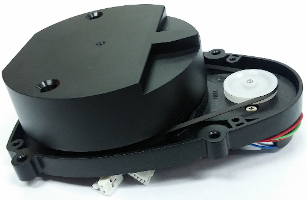
\includegraphics[height=5cm]{Bilder/lds_small.png}
			\caption{Der im Turtlebot 3 verbaute LiDAR-Sensor}
			\label{pic:lds_small}
		\end{figure}
	}
	
	\subsection{Raspberrry Pi}
	{
		Auf dem Turtlebot ist ein kleiner Computer, ein der Marke "Raspberry Pi" eingebaut. Standardmäßig handelt es sich dabei um das Modell der Reihe 3, welches jedoch aus Leistungsgründen mit einem Modell der 4. Generation ausgetauscht worden ist. Dieser Mikrocomputer stellt das Herzstück des Roboters dar und steuert alle Vorgänge. Wie ein jeder Computer besteht auch der Raspberry Pi aus einem Prozessor, Arbeitsspeicher, einer SD-Karte als Festplattenersatz und vielem mehr. Zwar stellt die Firma Raspberry auch eine graphische Benutzeroberfläche bereit, jedoch ist diese zur Programmierung nicht zweckführend, da diese Leistung verbraucht, welche für Berechnungen verwendet werden könnte. Aus diesem Grund verwende ich den Raspberry Pi mit einem einfachen Betriebssystem, welches nur eine Konsole anzeigt, um Leistung zu sparen.
	}
}